% !TeX encoding = UTF-8
% !TeX program = pdflatex
% !TeX spellcheck = it_IT

\documentclass[compress]{beamer}

%\setbeameroption{show only notes} % Decommentare per produrre l'output con solo le note.

\usepackage[italian]{babel}
\usepackage[utf8]{inputenc}
\usepackage{multirow}
\usepackage{minted}
\usepackage{wrapfig}

% Configurazione di minted, simile a quella della relazione.
\definecolor{LightGray}{gray}{0.9}
\setminted{
    linenos=true,
    autogobble,
    breaklines,
}

\usetheme[pageofpages=di,               % Stringa per separare la pagina corrente con il totale.
    alternativetitlepage=true,          % Prima pagina alternativa.
    titlepagelogo=presentation/assets/sapienza-logo, % Logo per la prima pagina.
    watermark=presentation/assets/watermark,         % Filigrana per tutte le pagine tranne la prima.
    watermarkheight=80px,
    watermarkheightmult=5]{Sapienza}    % Moltiplicatore dimensione del logo per la filigrana

\title{Progettazione e sviluppo delle API in linguaggio Go per il sistema di messaggistica domain-specific di SeismoCloud}
\author{Emanuele Petriglia}
\institute{Dipartimento di Informatica\\Università La Sapienza - Roma}
\date{20 luglio 2021}

\begin{document}

\begin{frame}[t,plain]
\titlepage
\end{frame}

\begin{frame}[c]{Obiettivo del tirocinio}
\begin{itemize}
\item \textbf{Necessità}: Attualmente in SeismoCloud gli utenti non possono interagire tra di loro.
\vspace{1em}
\item \textbf{Soluzione}: Creare uno spazio di interazione sociale basato sulle chat, concentrandosi sull'implementazione lato server e sulle API.
\end{itemize}
\end{frame}

\begin{frame}[c]{Passi affrontati}
\begin{itemize}
\item Cos'è SeismoCloud
\item Analisi requisiti
\item Progettazione
\item Implementazione
\item Conclusione
\end{itemize}

\note[item]{Specificare che i passi si affrontano in modo sommario.}
\end{frame}

\section{Cos'è SeismoCloud}

\begin{frame}[c]{SeismoCloud}
\begin{itemize}
\item È un sistema di rilevazione e allerta di terremoti;
\vspace{1em}
\item Il sistema è basato su una rete di sismometri (fissi e \textbf{mobili}) diffusi a livello nazionale;
\vspace{1em}
\item Lo scopo del sistema è l'\textbf{EEW} (Earthquake Early Warning).
\end{itemize}
\end{frame}

\begin{frame}[c]{Architettura della rete}
\begin{center}
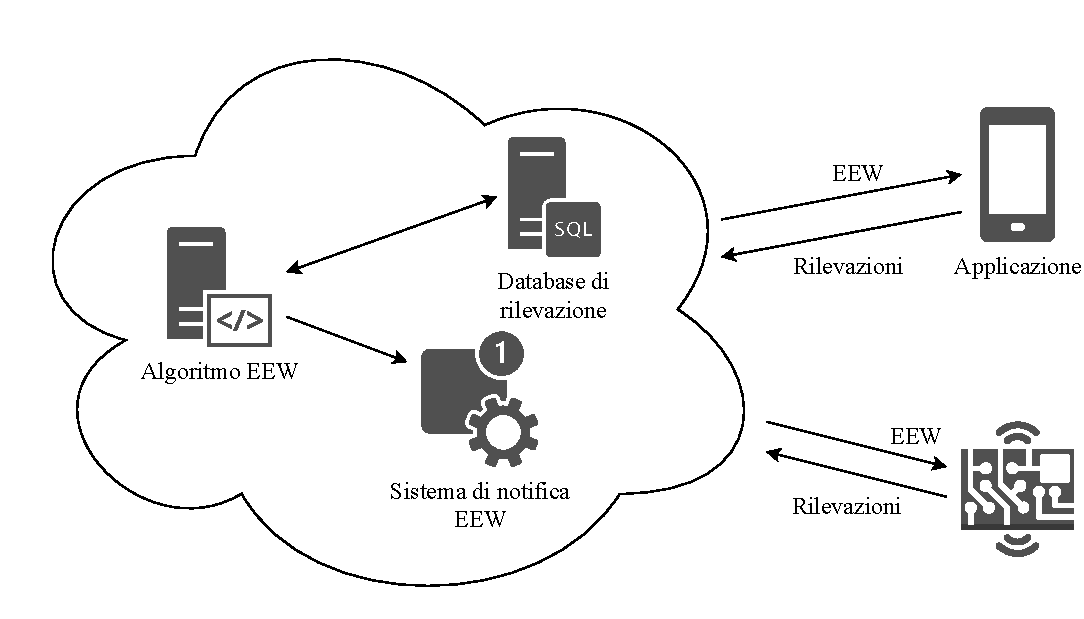
\includegraphics[width=\linewidth]{assets/01/rete.pdf}
\end{center}
\note[item]{Far vedere come funziona a grandi linee l'EEW.}
\end{frame}

\section{Analisi requisiti}

\begin{frame}[c]{Origine della funzionalità (1)}
\begin{center}
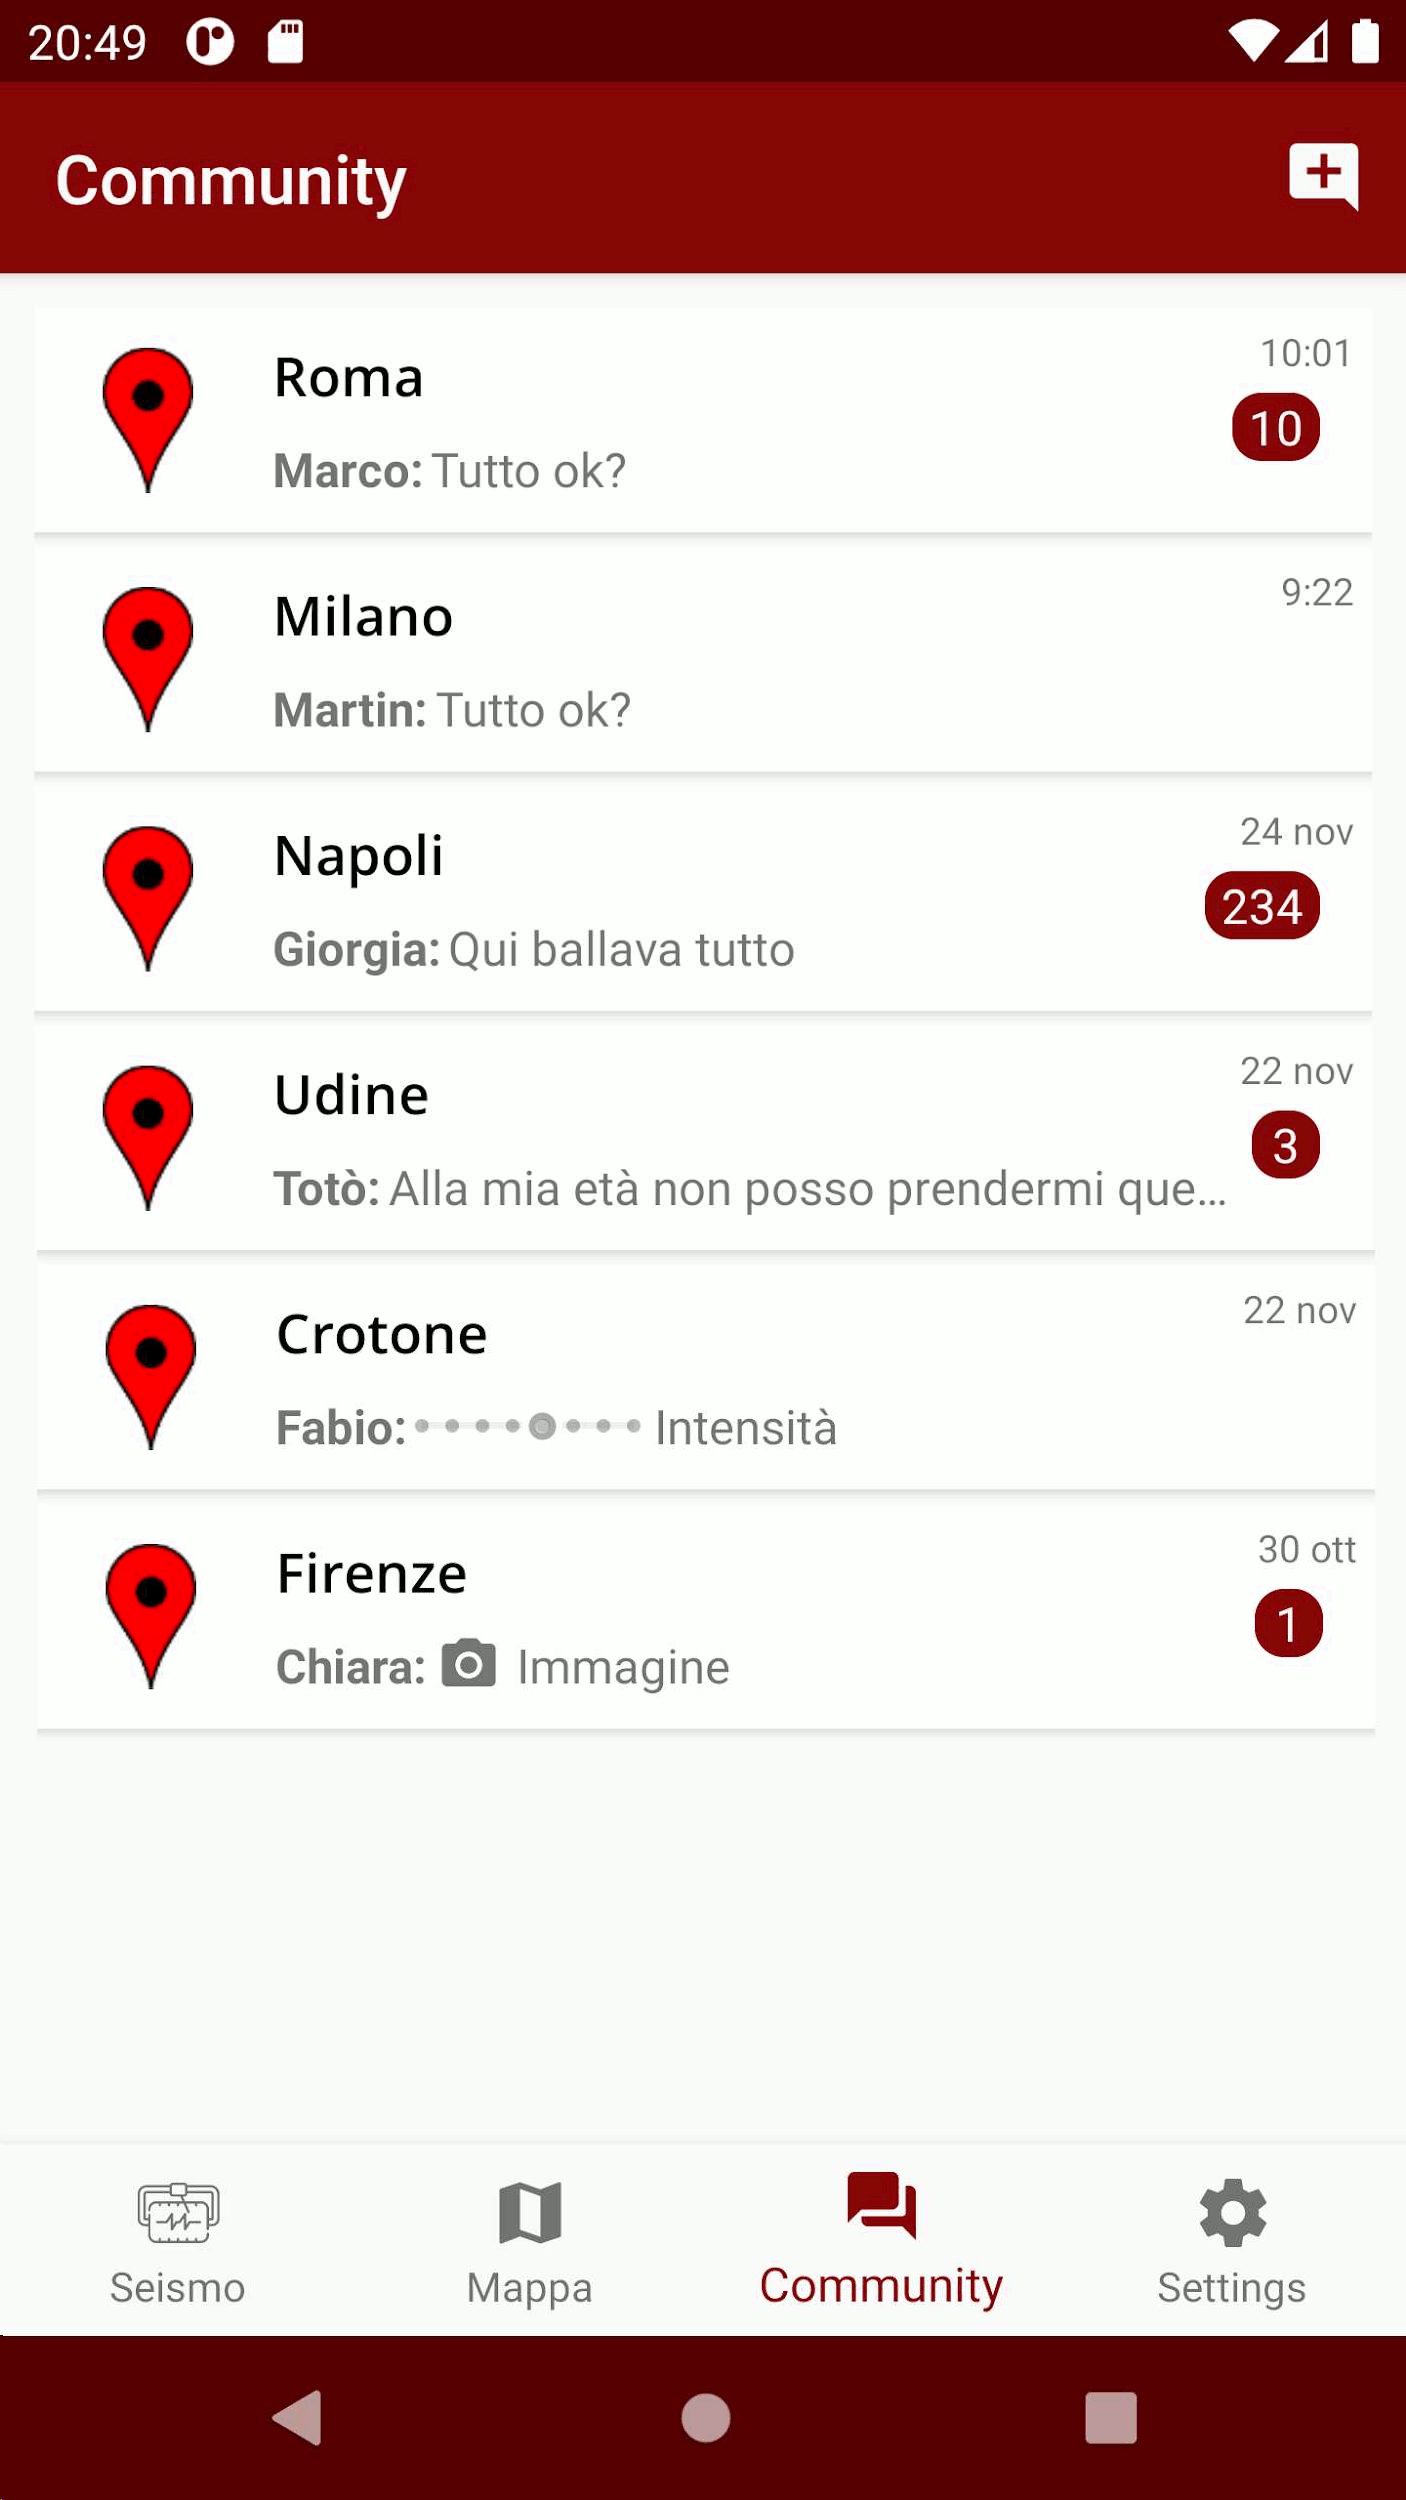
\includegraphics[scale=0.3]{assets/02/menu.png}
\hspace{2em}
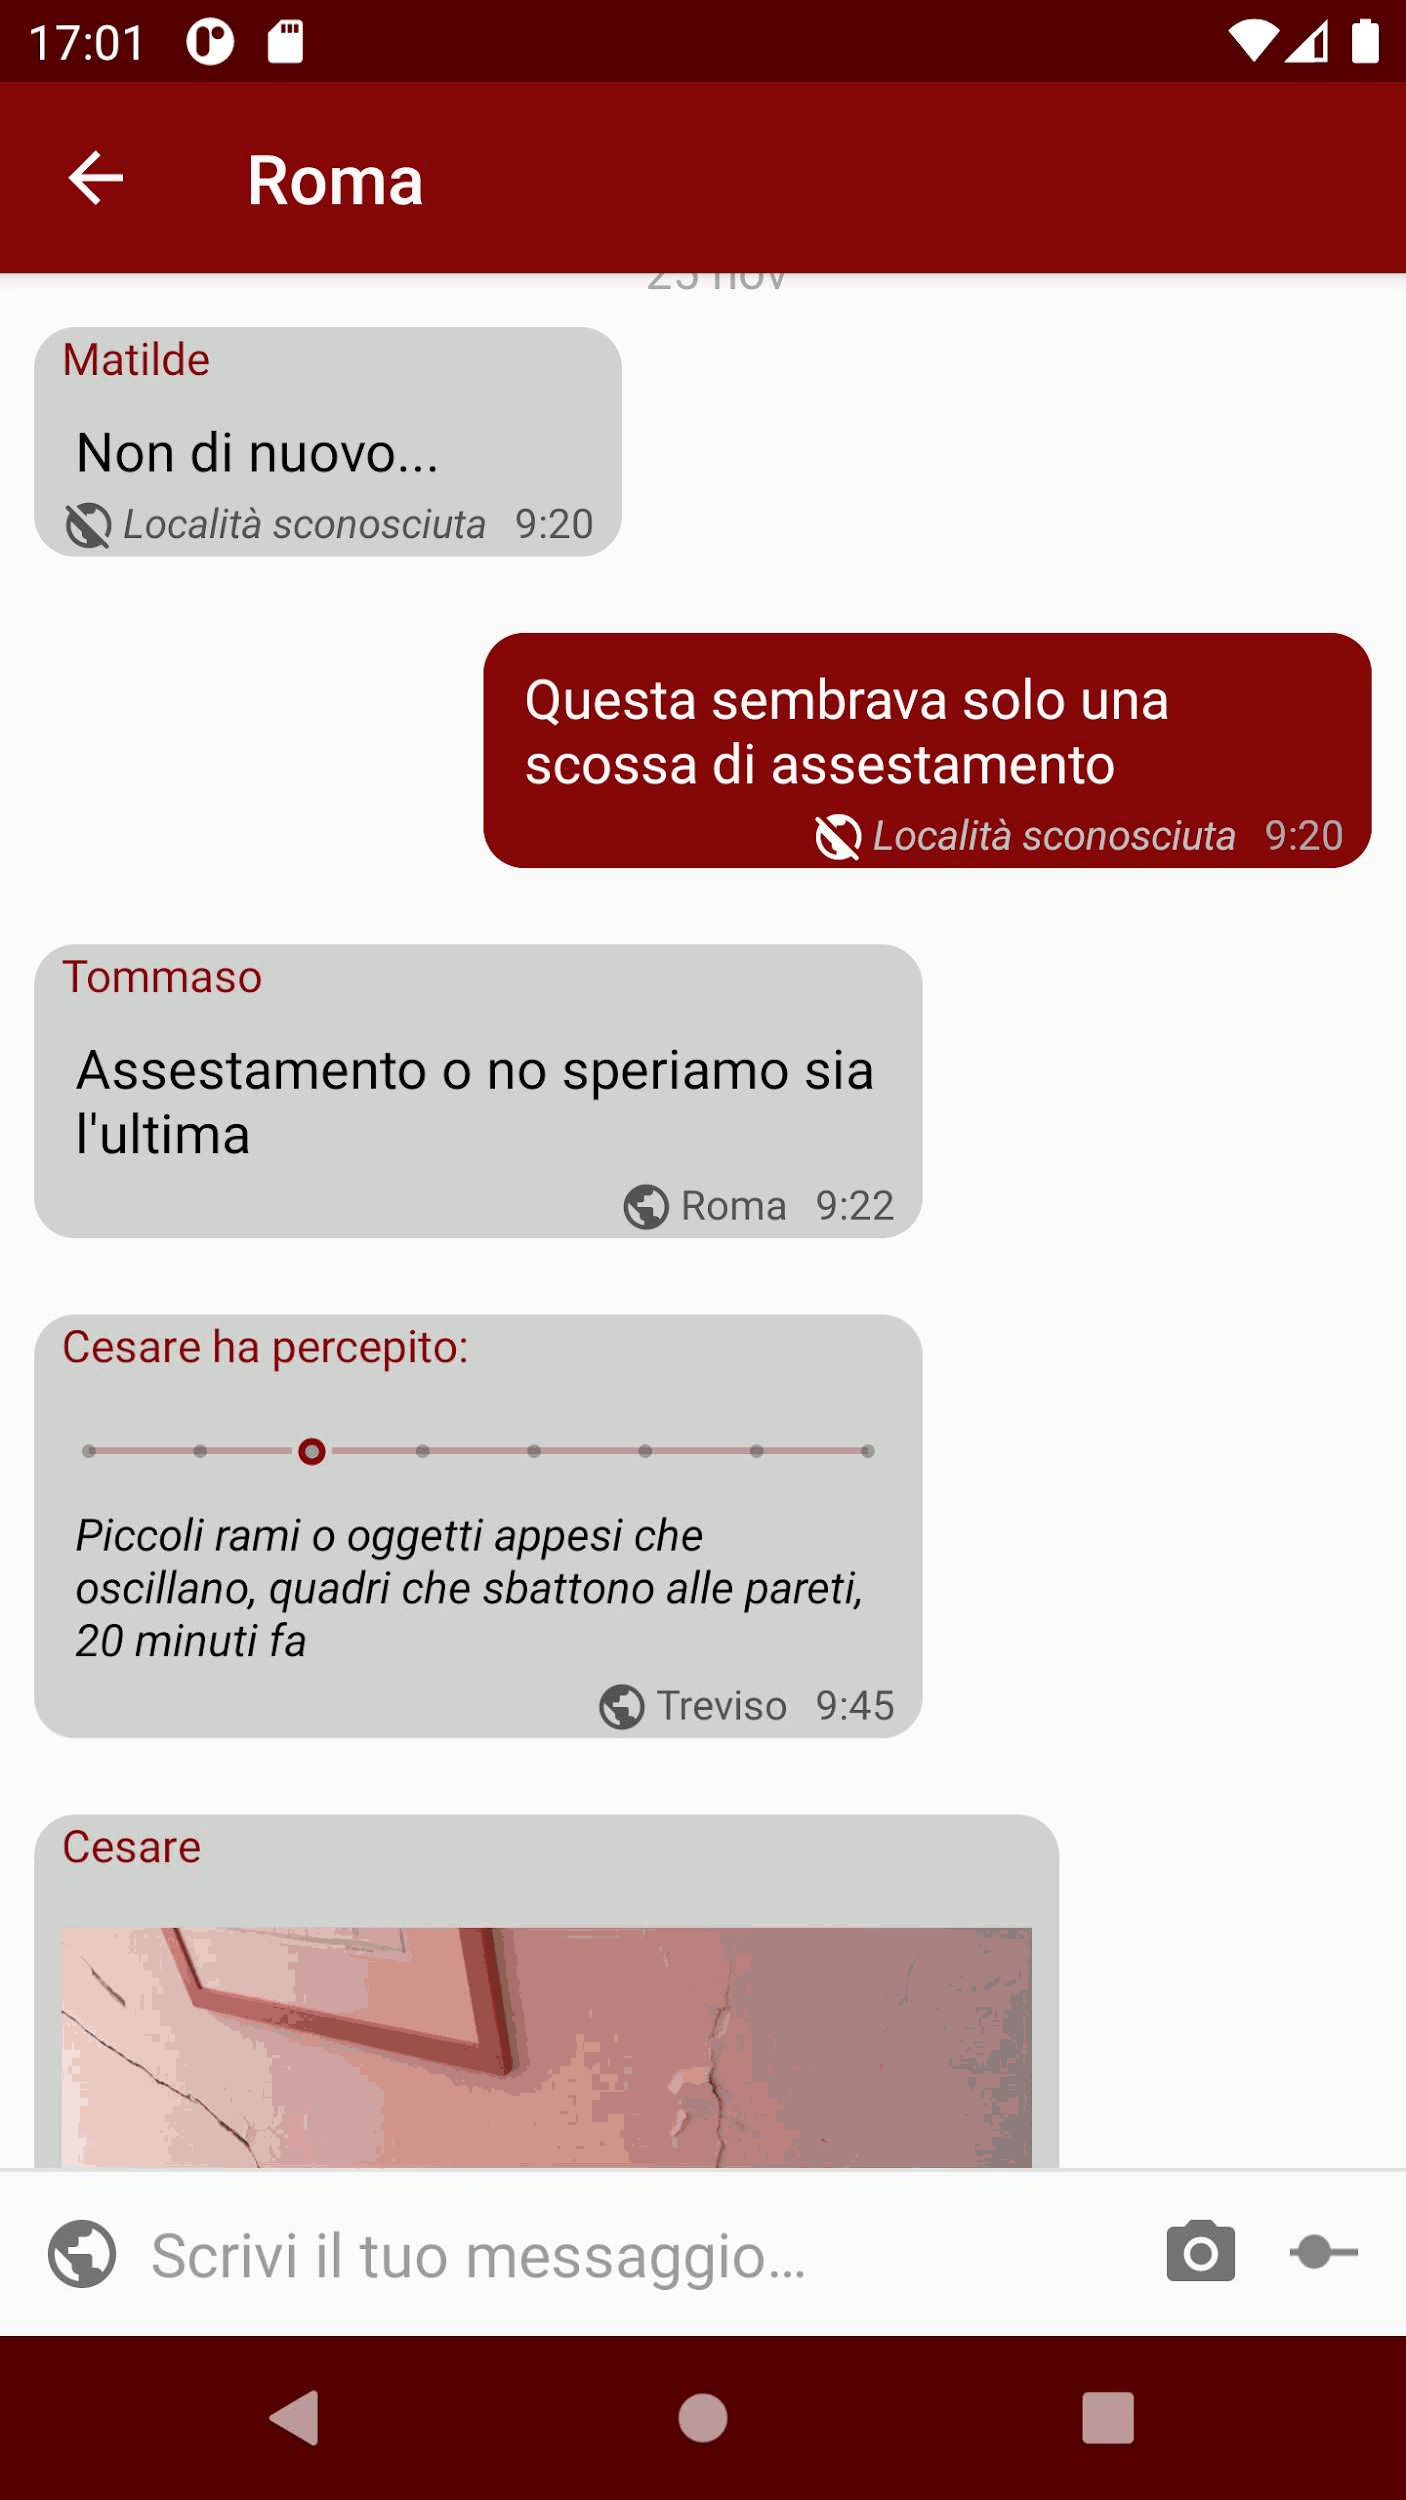
\includegraphics[scale=0.3]{assets/02/chat.png}
\end{center}
\note[item]{Specificare che le immagini sono prese dal lavoro di Michele Spina.}
\end{frame}

\begin{frame}[c]{Origine della funzionalità (2)}
\begin{center}
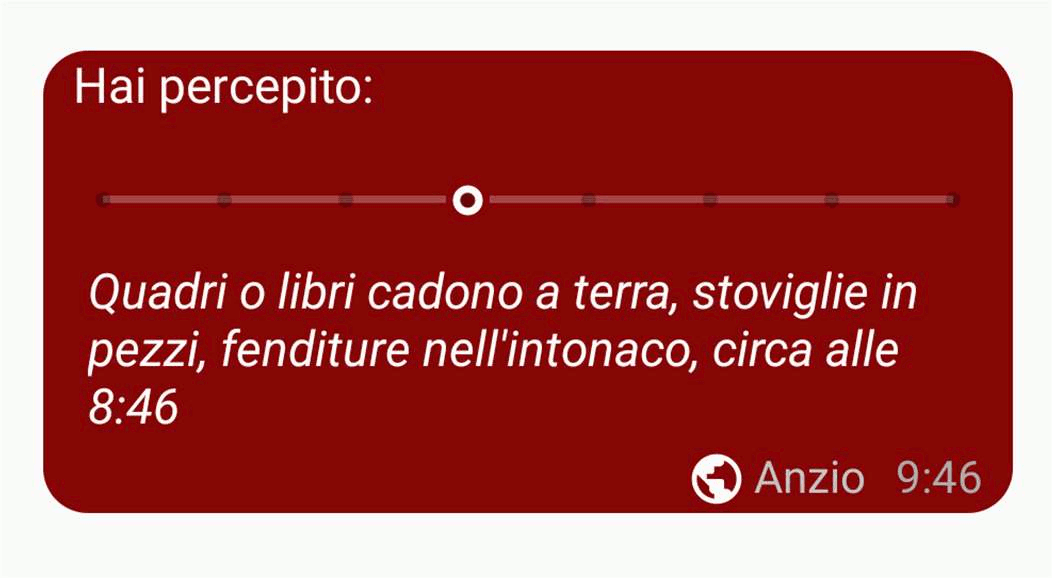
\includegraphics[scale=0.5]{assets/02/slider.png}
\hspace{2em}
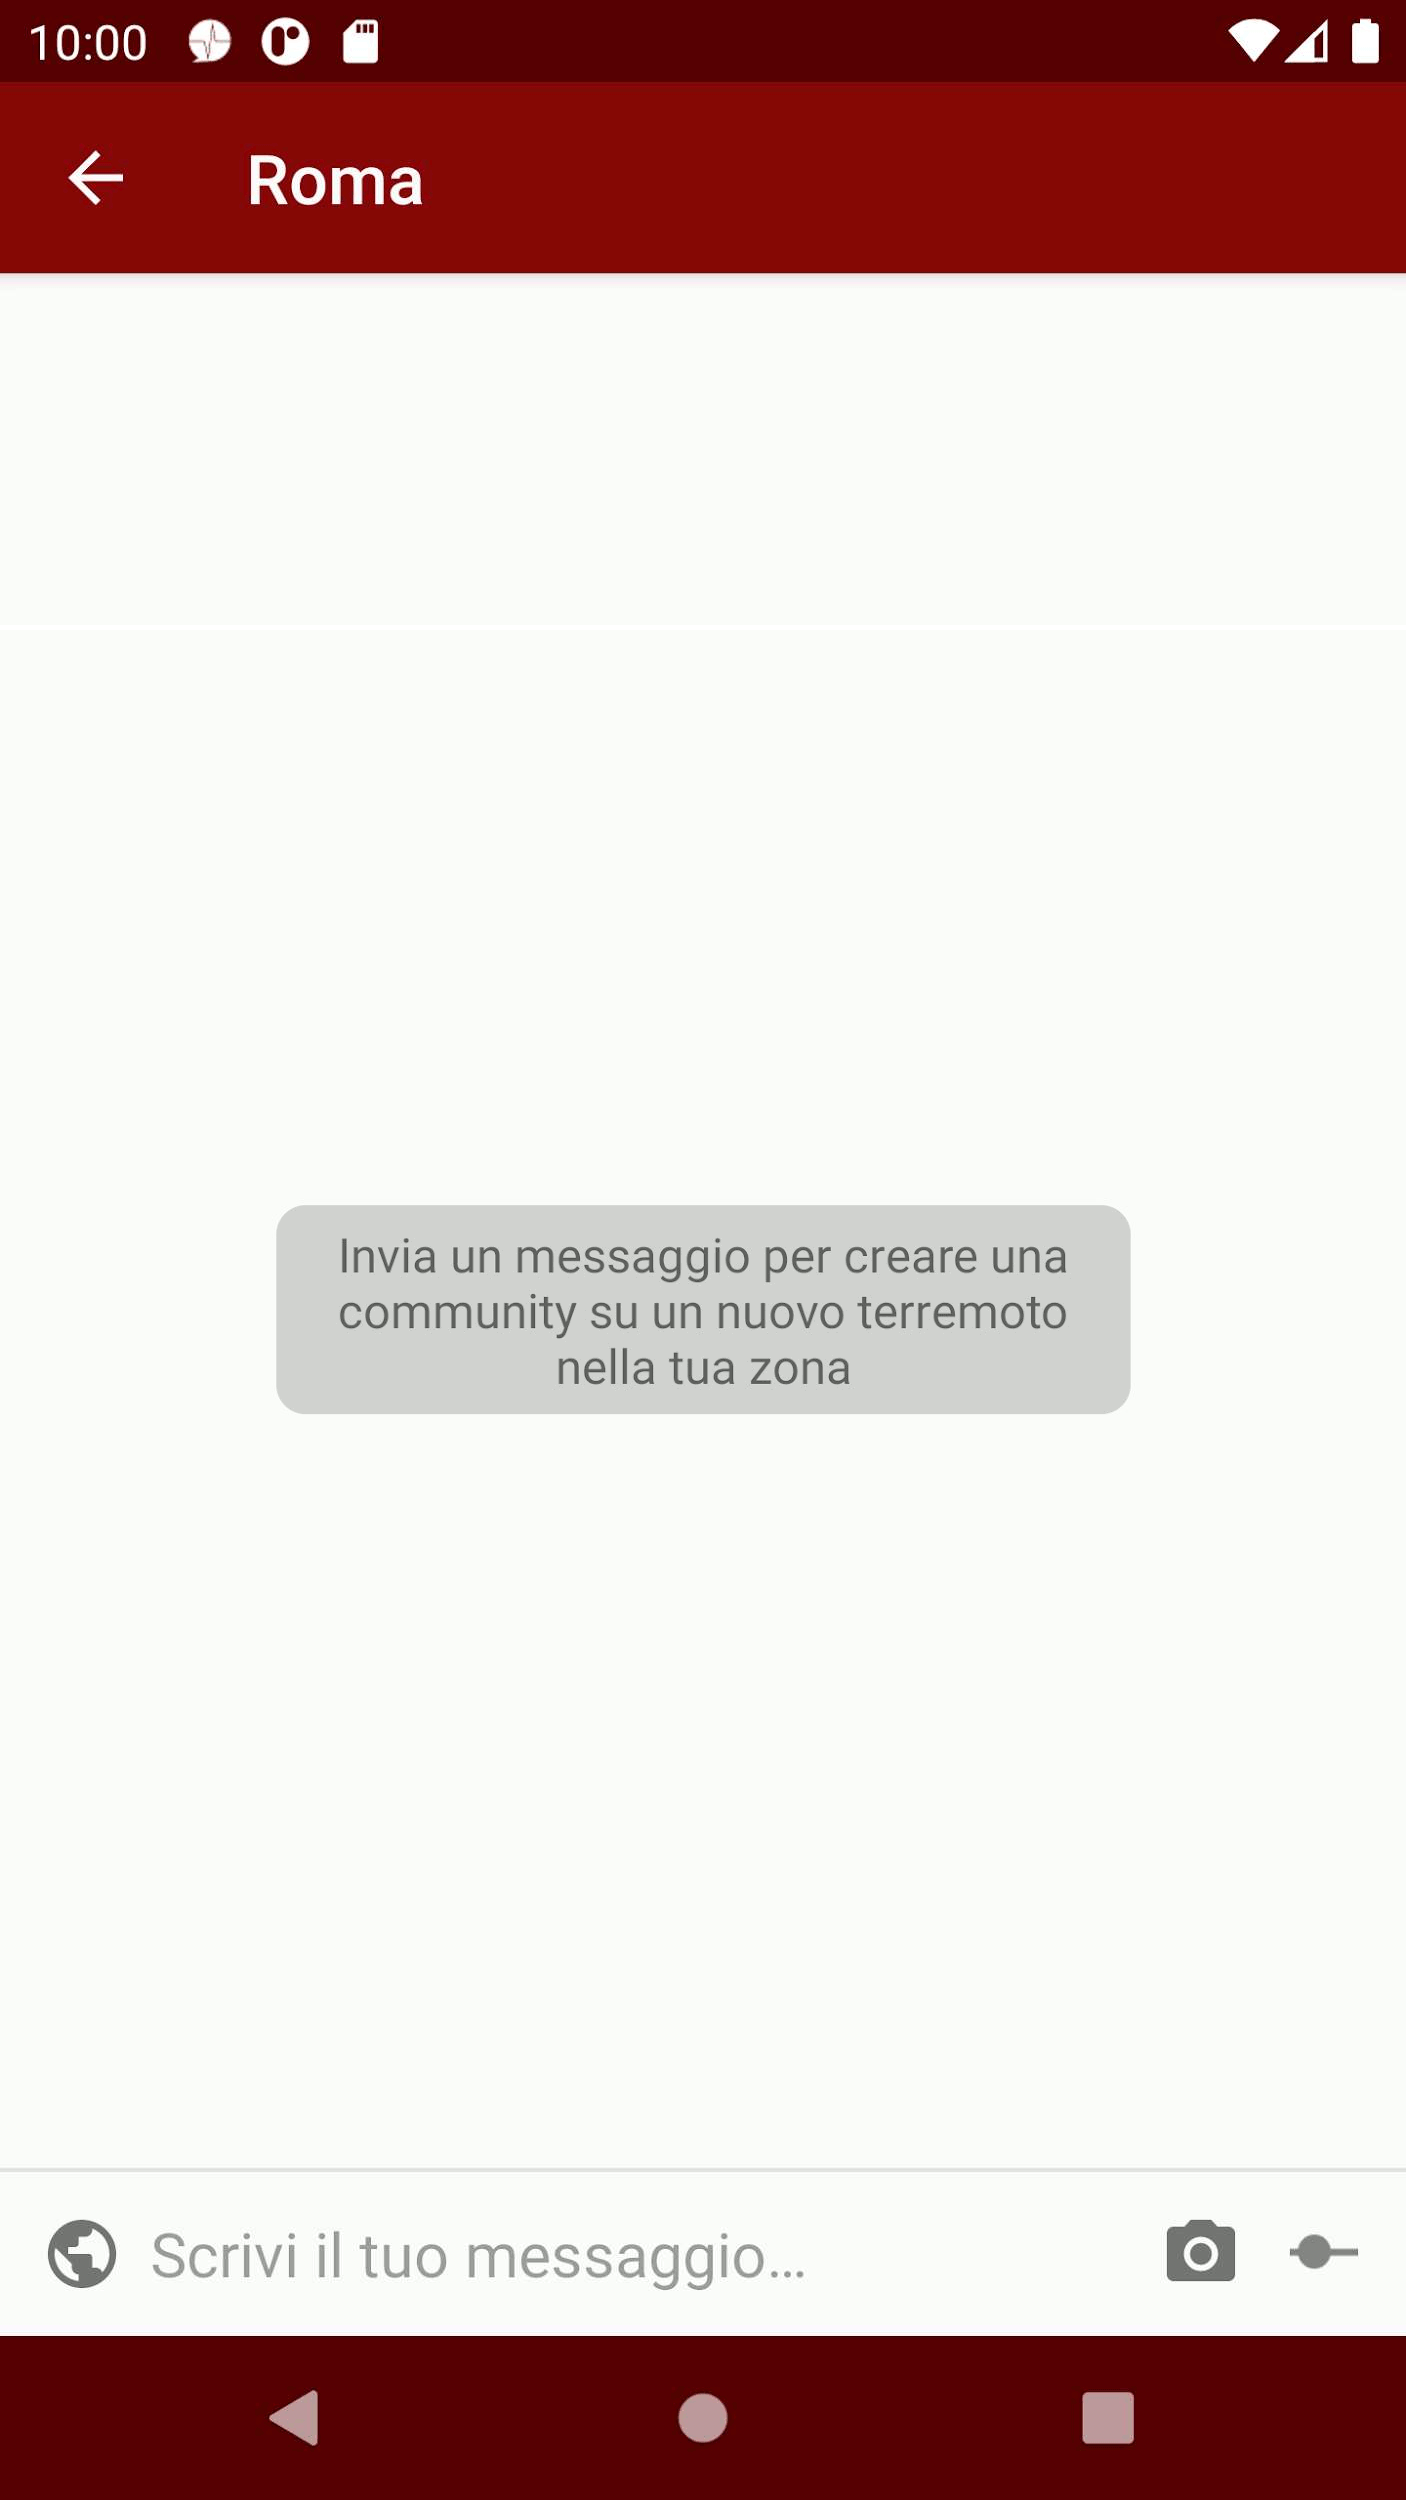
\includegraphics[scale=0.3]{assets/02/nuova_chat.png}
\end{center}
\end{frame}

\begin{frame}[c]{Caratteristiche}
\begin{itemize}
\item \textbf{Chat}: creazione, chiusura/verifica, elenco chat e messaggi, posizione geografica, nome;
\vspace{0.5em}
\item \textbf{Messaggio}: tipologie (testuale, fotografico, slider), invio su chat aperte;
\vspace{0.5em}
\item \textbf{Utente}: nome utente personale;
\vspace{0.5em}
\item \textbf{Sottoscrizione}: notifiche, iscrizione automatica alla creazione.
\end{itemize}
\end{frame}

\section{Progettazione}

\begin{frame}[c]{REST e OpenAPI}
\begin{itemize}
\item Stile architetturale \textit{REST}: basato su HTTP, concetto di risorsa e di collezione, con un URI per l'identificazione e JSON per la rappresentazione.
\vspace{0.5em}
\item Specifica \textit{OpenAPI}: utilizzata per descrivere le API.
\begin{center}
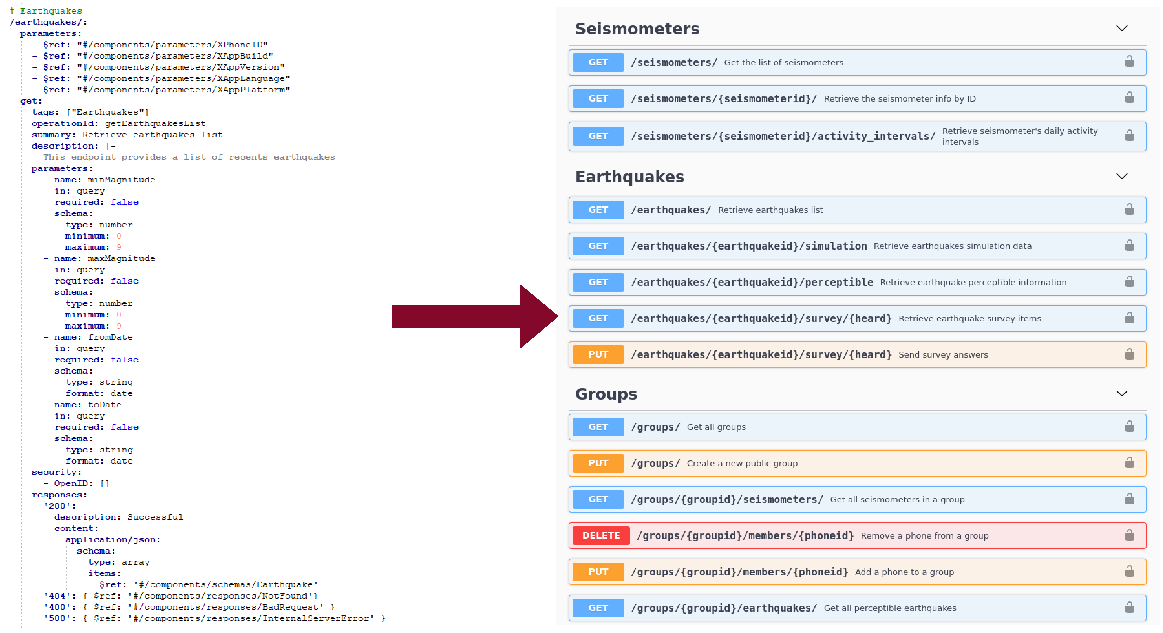
\includegraphics[scale=0.5]{presentation/assets/codice2openapi.pdf}
\end{center}
\end{itemize}
\note[item]{Dire in due parole cos'è REST e cosa si intende per API.}
\note[item]{Far vedere la foto e spiegarla brevemente.}
\end{frame}

\begin{frame}[c]{API progettate}
\begin{table}[ht!]
\centering
\begin{tabular}{c|c|c}
\textbf{Risorsa} & \textbf{Metodo} & \textbf{URL} \\
\hline
\multirow{2}{*}{Chat} & GET & /chats/ \\
    & PUT & /chats/ \\
\hline
\multirow{2}{*}{Messaggi} & PUT & /chats/\{chatid\}/messages/ \\
    & GET & /chats/\{chatid\}/messages/ \\
\hline
Immagini & GET & /images/\{imageid\} \\
\hline
\multirow{2}{*}{Utenti} & GET & /me/username \\
    & PUT & /me/username \\
\hline
\multirow{2}{*}{Sottoscrizioni} & DELETE & /me/chats/subscribed/\{chatid\} \\
    & PUT & /me/chats/subscribed/\{chatid\}
\end{tabular}
\end{table}
\note[item]{Differenza tra risorsa e collezione.}
\note[item]{Le uniche API complesse sono la creazione del messaggio e la creazione delle chat.}
\end{frame}

\begin{frame}[c]{Diagramma concettuale del database}
\begin{center}
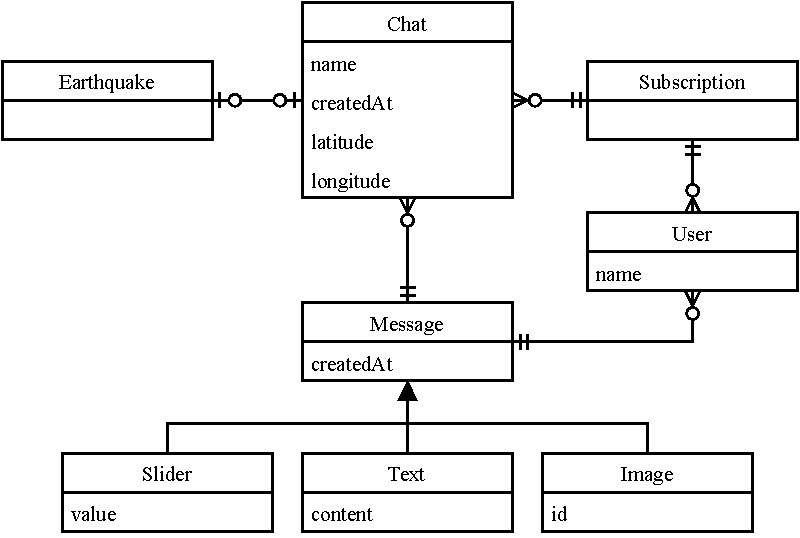
\includegraphics[scale=0.7]{assets/03/concettuale.pdf}
\end{center}
\end{frame}

\section{Implementazione}

\begin{frame}[c]{Componenti interessati}
\begin{center}
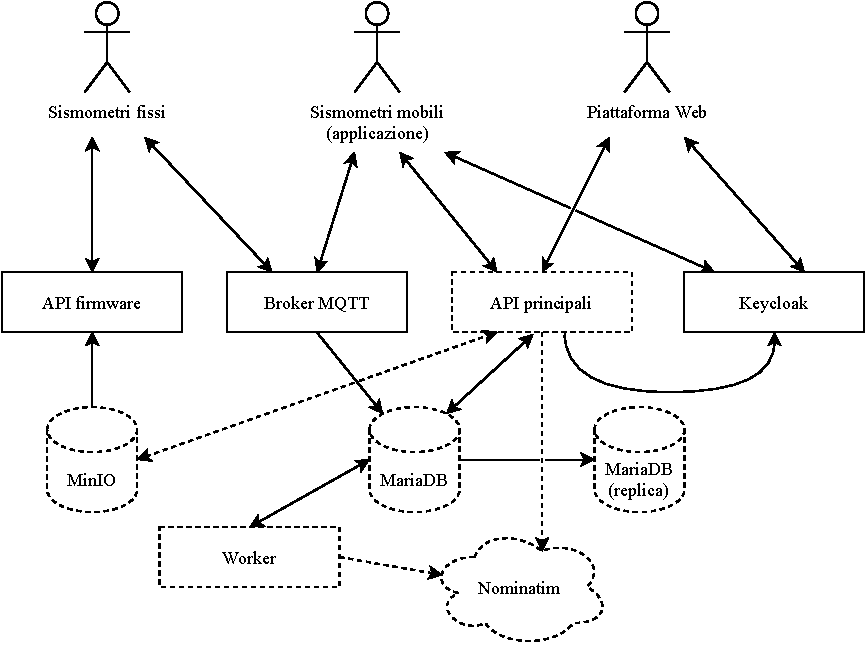
\includegraphics[width=0.9\linewidth]{assets/04/architettura-modify.pdf}
\end{center}
\end{frame}

\begin{frame}[c]{Linguaggio Go}
\begin{itemize}
\item È un linguaggio di programmazione tipizzato staticamente, multi-paradigma, sintatticamente simile al C;
\item Non è prettamente orientato agli oggetti;
\item Predominanza delle strutture, interfacce (diverse da Java) e loro composizione.
\end{itemize}

\vspace{1em}

Nel lato server di SeismoCloud è utilizzato per implementare le API e il Worker.

\end{frame}

\begin{frame}[c]{Gestione di una richiesta HTTP}
\begin{center}
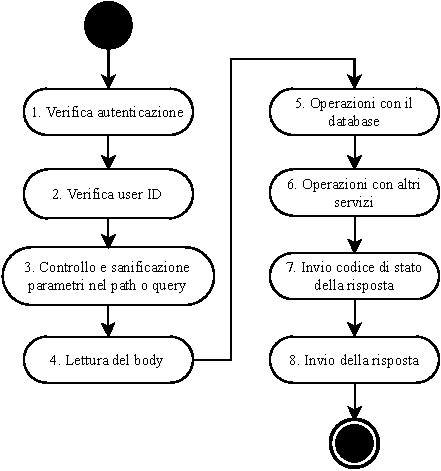
\includegraphics[scale=0.85]{assets/04/operazioni-api.pdf}
\end{center}
\end{frame}

\begin{frame}[fragile,c]{Implementazione di \texttt{GET /me/username}}
\begin{minted}[fontsize=\tiny]{go}
func (rt *_router) getUsername(w http.ResponseWriter, r *http.Request, ps httprouter.Params, ctx reqcontext.RequestContext) {
	if ctx.UserID == uuid.Nil {
		ctx.Logger.Info("getUsername: userid nil")
		w.WriteHeader(http.StatusBadRequest)
		return
	}

	username, err := rt.DB.GetUsername(ctx.UserID)
	if err != nil {
		switch err {
		case database.ErrNoUsername:
			ctx.Logger.Info("getUsername: user doesn't have a username")
			w.WriteHeader(StatusUsernameRequired)
		default:
			ctx.Logger.WithError(err).Error("getUsername: can't get username")
			w.WriteHeader(http.StatusInternalServerError)
		}
		return
	}

	if _, err := w.Write([]byte(username)); err != nil {
		ctx.Logger.WithError(err).Error("getUsername: can't write body")
	}
}
\end{minted}
\note[item]{Dire che le operazioni sul DB si fanno nel metodo \texttt{GetUsername}.}
\end{frame}

\begin{frame}[c]{Compiti periodici nel Worker}
\begin{itemize}
\item \texttt{closeChats}: eseguito in ogni minuto, chiude le chat che non sono state associate ad alcun terremoto entro le 24 ore;
\vspace{1em}
\item \texttt{matchChats}: eseguito in ogni minuto, tenta di assegnare un terremoto a una chat non verificata e ancora aperta.
\end{itemize}
\end{frame}

\section{Conclusione}

\begin{frame}[c]{Risultato}
Il sistema è in una versione minimale ma funzionante (\textit{minimum viable product}, MVP). In questo modo si possono ottenere feedback dagli utenti per veicolare al meglio gli sviluppi futuri.

\vspace{2em}

Manca l'integrazione con i client, sia per le interfacce  utente che per le API, prima di mettere in produzione il sistema.
\end{frame}

\begin{frame}[c]{Sviluppi futuri}
\begin{enumerate}
\item Miglioramento dell'algoritmo di creazione delle chat;
\item Test più robusti di varia tipologia (integrazione, carico, unitari...);
\item Realizzazione del sistema delle notifiche;
\item Istanza personale di Nominatim.
\end{enumerate}
\end{frame}

\revslide{Grazie}

\end{document}
